\subsection{Registrar Entrada de Vehículo}
En la figura \ref{fig:Diagrama de Secuencia - Registrar Entrada de Vehículo} se plasma el diagrama de secuencia que corresponde al registro de entrada de un vehículo al taller. El Mecánico (usuario) solicitará esta opción al sistema y este mismo le solicitará por medio de un formulario los datos necesarios para hacer el registro en la base de datos. Hay dos variantes en cuanto a la información ingresada: 
\begin{itemize}
	\item \textbf{Información válida:} Los datos que ha ingresado el usuario son válidos, es decir, que todos los campos han sido llenados y el formato del campo ingresado es el correcto. 
	\item \textbf{Información no válida:} Los datos que ha ingresado el usuario no son correctos. 
\end{itemize}
\begin{figure}[!h]
	\centering
	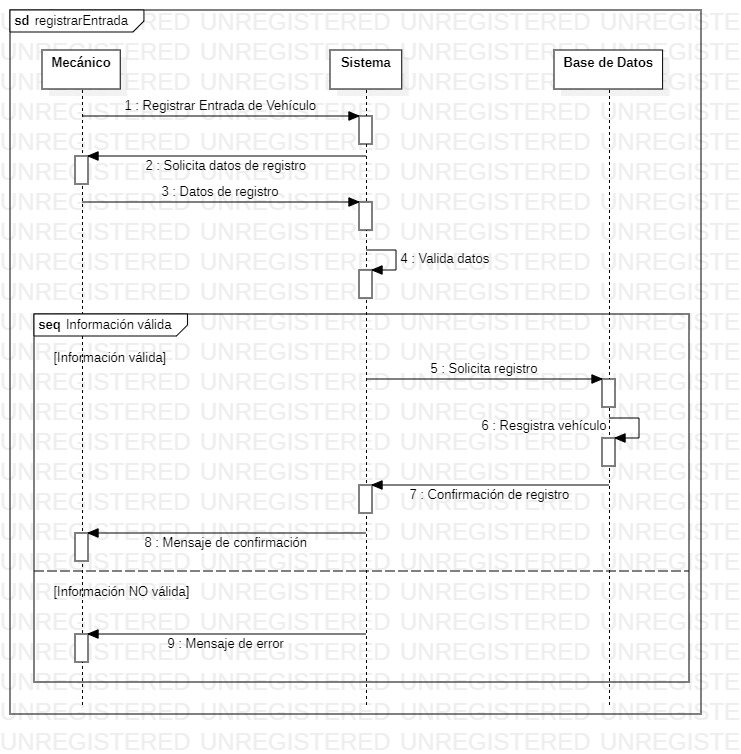
\includegraphics[width=0.8\textwidth]{./diseno/vprocesos/imagenes/registrarEntrada}
	\caption{Diagrama de Secuencia - Registrar Entrada de Vehículo}
	\label{fig:Diagrama de Secuencia - Registrar Entrada de Vehículo}
\end{figure}